\documentclass{article}
\usepackage{amsmath}
\usepackage{graphicx}
\begin{document}
\title{CNN}
\date{ }
\maketitle
\section{size of feature map}
given input size,padding,filter size and stride,we can determine size of feature map:$$size\,of\,feature\,map=\lfloor\frac{inputsize+2*padding-filter\,size}{stride}+1\rfloor $$By saying size,it refers to length of every index of the matrix being considered.
\par eg.Say we have that input size is $h\times w\times c$,filter size is $f_1\times f_2\times f_3$,padding $p$ and stride $s$.Then size of feature map is $a\times b\times c$ with
\begin{align*}
	&a=\lfloor\frac{h+2p-f_1}{s}+1\rfloor\\
	&b=\lfloor\frac{w+2p-f_2}{s}+1\rfloor\\
	&c=\lfloor\frac{c+2p-f_3}{s}+1\rfloor
\end{align*}
In a lot of cases,"same" padding is taken into acount in order to maintain equality between input size and output size.To do this,padding and stride are particularly chosen so that the left hand size of the fomular will be exactly equal to size of input.
\section{image recognition(RBG)}
Input size = height$\times$width$\times$channels(corresponding to R,B,G).It is required number of filters is equal to the number of channels and add up all the convolution output to get a feature map.Conceptual diagram reads
\begin{figure}[htbp]
	\centering
	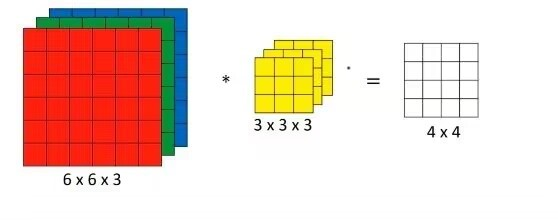
\includegraphics[width=0.5\textwidth]{1.jpg}
	\caption{RBG's filters}
\end{figure}
To actually extract more features from input,more than a set of kernels(filters) are needed.With multiple set of kernels it comes multiple set of feature maps that will eventually form a matrix with higher dimension.
\par eg.Let input size be $6\times6\times3$,kernel size be $(3\time3\time3)*2$(2 set of filters,with each possessing 3 filters sizing $3\time3$),padding be $0$ and stride be $1$.
In this example,two convolution jobs are to be done.According to the formular,one can calculate the size of each feature maps(2 in total).
\begin{align*}
	&convolution_1\rightarrow4\times4\;matrix\\
	&convolution_2\rightarrow4\times4\;matrix\\
	&gather\;two\;convolutional\;results\rightarrow4\times4\times2\;matrix
\end{align*}
\section{bias}
When feature map is finally produced,add a bias term to it elementwise with each added with the same bias.Different feature map is assigned with different biases.
\section{layer}
A convolutional layer in CNN shall include the following building blocks
\par (1) convolution between kenels and input matrix.
\par (2) biases for each feature map
\par (3) matrix of higher dimension formed by all convolutional results.
\par (4) Relu function applied to matrix in (3).
\section{number of parameters}
The number of parameters in one layer is determined its bias and kenels.A general formular that finds this number is
$$P=B+WK$$
where $P$ indicates number of parameters,$B$ represents number of different biases,$WK$ counts number of weights of all kernels.
\par eg.In one particular layer,it finds 10 filters sized $3\times3\times3$,then the number of parameters needed in this layer is$$10+10*(3*3*3)$$
The $10$ shows in at the head of the expression is what is referred to as $B$ in the formular and the latter is $WK$.
\section{systematic process in one layer}
Let $l$ be ordinal of convoltutional layer.Elements related to layer $l^{th}$ are
\begin{align*}
	&f^{[l]}=filter\;size(In\;actuality\;,filter\;is\;mostly\;designed\;as\;square)\\
	&p^{[l]}=padding\\
	&s^{[l]}=stride\\
	&n^{[l]}_C=number\;of\;channels\\
	&N^{[l]}=number\;of\;sets\;of\;kernels\\
	&Input:n^{[l-1]}_H\times n^{[l-1]}_W\times n^{[l-1]}_C\\
	&Output:n^{[l]}_H\times n^{[l]}_W\times n^{[l]}_C\\
	&Kernel:f^{[l]}\times f^{[l]}\times n^{[l-1]}_C\\
\end{align*}
With these,output size of layer $l^{th}$ is automatically
$$n^{[l]}_k=\lfloor\frac{n^{[l-1]}+2p^{[l]}-f^{[l]}}{s^{[l]}+1}\rfloor,k=H,W$$
while channel of this layer is preset as $n^{[l]}_C$.
This can be visualized via a diagrammatic instance
\begin{figure}[htbp]
	\centering
	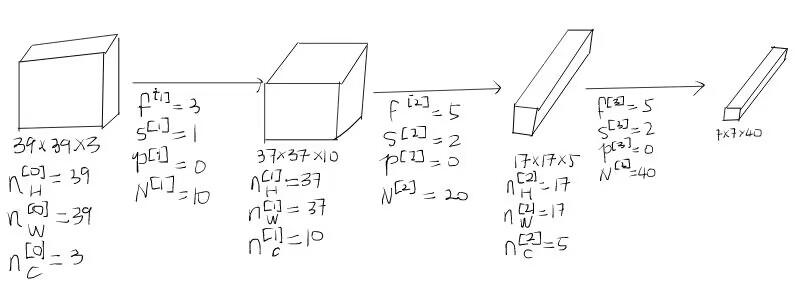
\includegraphics[width=0.8\textwidth]{2.jpg}
	\caption{visulization of systematic process}
\end{figure}
\vspace{\textheight}
\section{Pooling(max pooling)}
Max pooling is almost identical to convolution except that it uses kernnel to max-pick the element in selected window.An instant example will be the following diagram,
\begin{figure}[htbp]
	\centering
	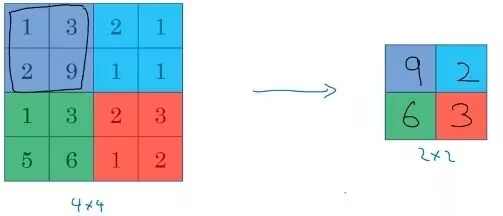
\includegraphics[width=0.6\textwidth]{3.jpg}
	\caption{max pooling}
\end{figure}
where the pooling filter has size $4\times4$ and the first sliding window picks out 9 as it is the biggest in current window.
\par parameters of a pooling kernel should include:(1)filter sizes;(2)stride;(3)and generally no padding and they are preset so need not to learn.
\par If the pooling object is of multi-channels then it shall do max pooling channel-wise.Size of the output of pooling can be calculated the way output size of convolution is calculated.
\par eg.Let a pooling filter size $3\times3$ and input size $5\times5$,then pooling process can be explained also by a diagram:
\begin{figure}[htbp]
	\centering
	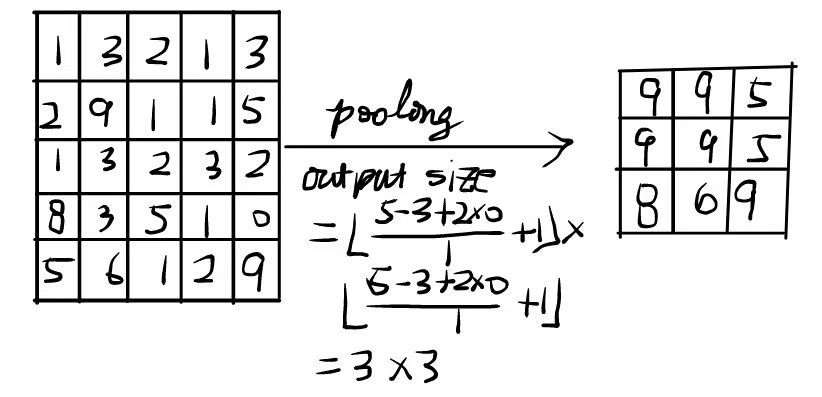
\includegraphics[width=0.6\textwidth]{4.jpg}
	\caption{pooling process}
\end{figure}
\section{Building blocks of CNN}
To construct a CNN,one must consider the following three types of layers
\par (1)Convolutional layer (CONV)
\par (2)Pooling layer (POOL)
\par (3)Fully connected layer,like softmax layer (FC) 
As datas go deeper in CNN,matrixes shall tend to have smaller size in one channel but have more channels.
\section{classic CNNs}
\subsection{LeNet}
LeNet is created to regconize grey scale image sized $32\times32$.It can be illustrated as a diagram
\begin{figure}[htbp]
	\centering
	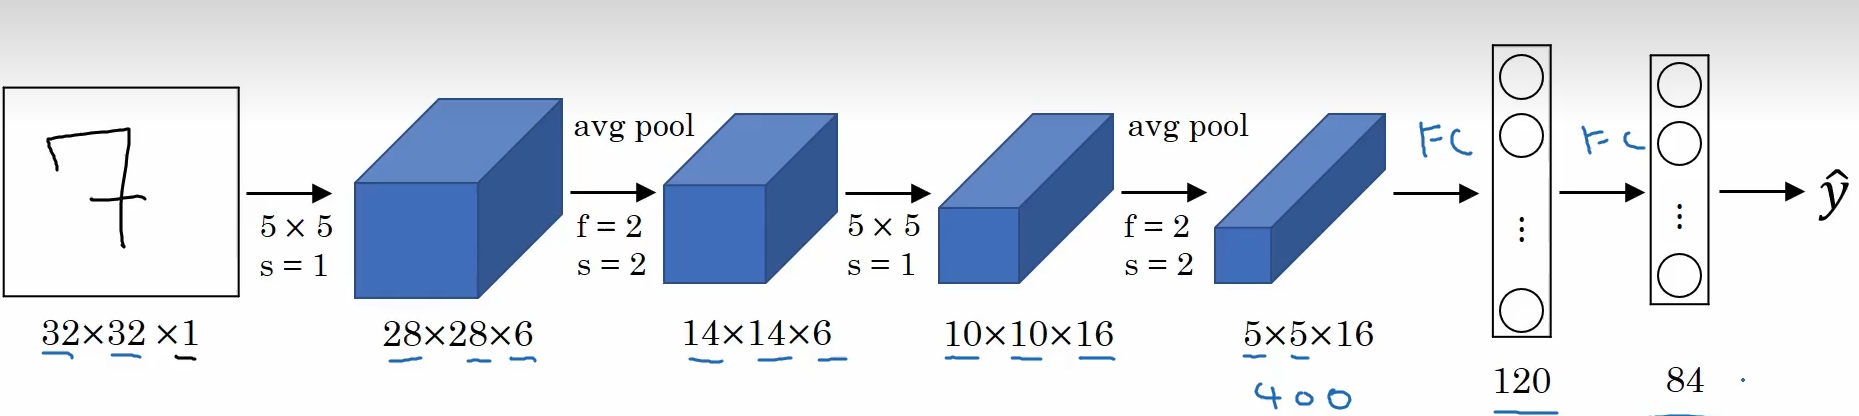
\includegraphics[width=0.7\textwidth]{5.png}
	\caption{LeNet flow chart}
\end{figure}
\vspace{0.1\textheight}
\subsection{AlexNet}
AlexNet can cope with RBG digits.In its original design,it takes in a image of 3 channels with each channel sized $227\times227$,and it can be demenstrated by a diagram
\begin{figure}[htbp]
	\centering
	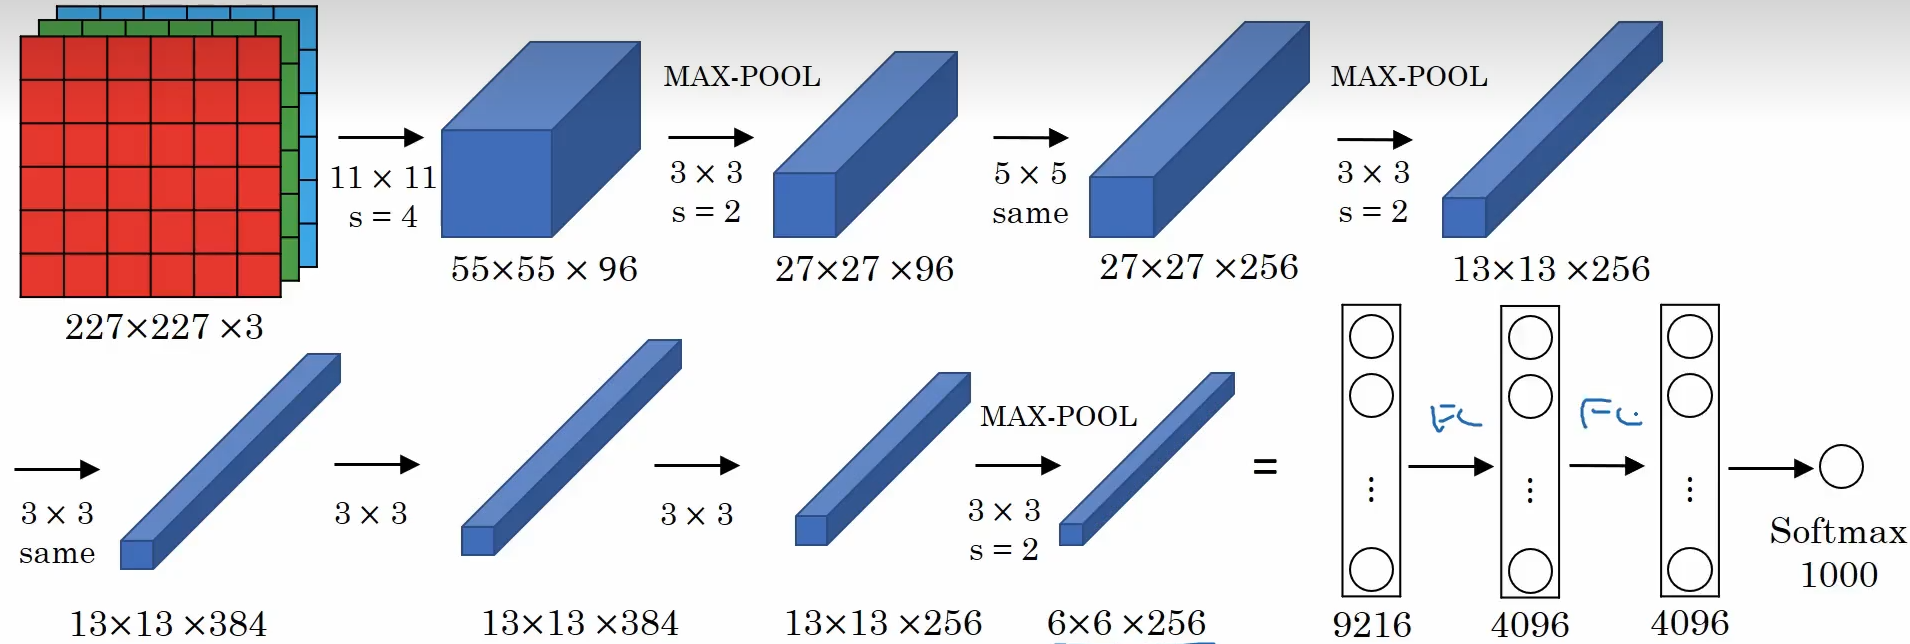
\includegraphics[width=0.7\textwidth]{6.png}
	\caption{AlexNet flow chat}
\end{figure}
\vspace{0.1\textheight}
\subsection{VGG-16}
VGG-16 has simple and regular pattern,however,with gigantic size of parameter set.It is also capable of RBG digits recognition.The "16" in its name suggests that there are 16 layers with weights within its structure.For the sake of convinence,let CONV denotes one convolutional layer whose filter size is $3\times3$,stride is $1$ and padding is $same$,also let POOL denotes a max pooling whose filter size is $2\times2$ and stride is $2$.The following is the diagram
\begin{figure}[htbp]
	\centering
	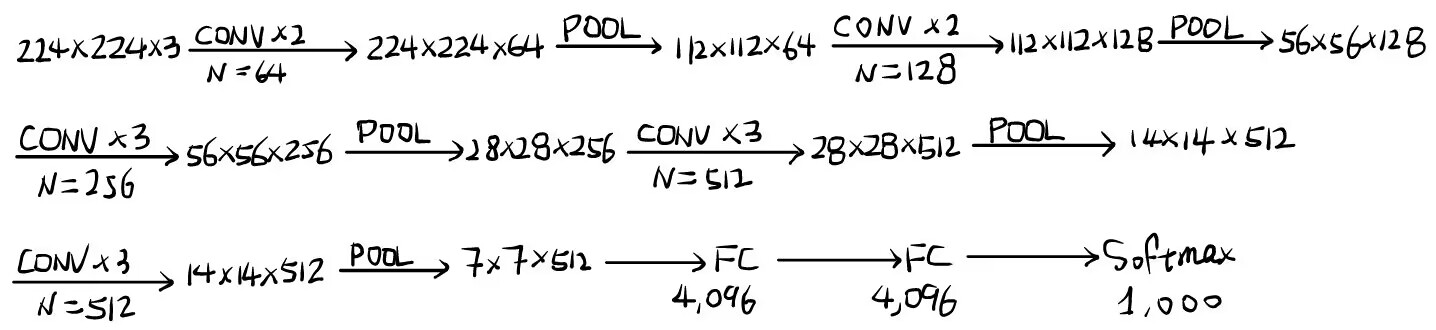
\includegraphics[width=0.7\textwidth]{7.jpg}
	\caption{VGG-16 flow chart}
\end{figure}
\section{Residual Network}
RN(Residual Network) allows datas to skip layer to reach its next layer.As is known to all,a usual and plain network looks like
\begin{figure}[htbp]
	\centering
	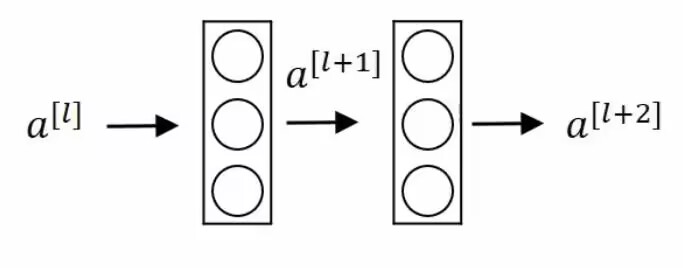
\includegraphics[width=0.7\textwidth]{8.jpg}
	\caption{plain network}
\end{figure}
The algebra detail goes:
\par In layer $(l+1)^{th}$  where $a^{[l]}$ comes in and $a^{[l+1]}$ goes out,there is a linear function $z^{[l+1]}=W^{[l+1]}a^{[l]}+b^{[l+1]}$ and a activation function $h(x)$ such that $a^{[l+1]}=h(z^{[l+1]})$.Similar algebra takes place in layer $(l+2)^{th}$.
\par Now to Residualize this network,allowing $a^{[l]}$ to jump into layer $(l+2)^{th}$ while still also entering layer $(l+1)^{th}$.Consequently,the algebra process becomes
\begin{align*}
	&z^{[l+1]}=W^{[l+1]}a^{[l]}+b^{[l+1]},a^{[l+1]}=h(z^{[l+1]})\\
	&z^{[l+2]}=W^{[l+2]}a^{[l+1]}+b^{[l+2]},a^{[l+2]}=h(z^{[l+2]}+a^{[l]})
\end{align*}
In this setting,it is required that $z^{[l+2]}$ and $a^{[l]}$ share the same dimension otherwise $a^{[l]}$ should be multiplied by a matrix(either fixed or to learn) to tailor its dimension.
\vspace{0.4\textheight}
\par As a visual aid,its conceptual diagram looks like
\begin{figure}[htbp]
	\centering
	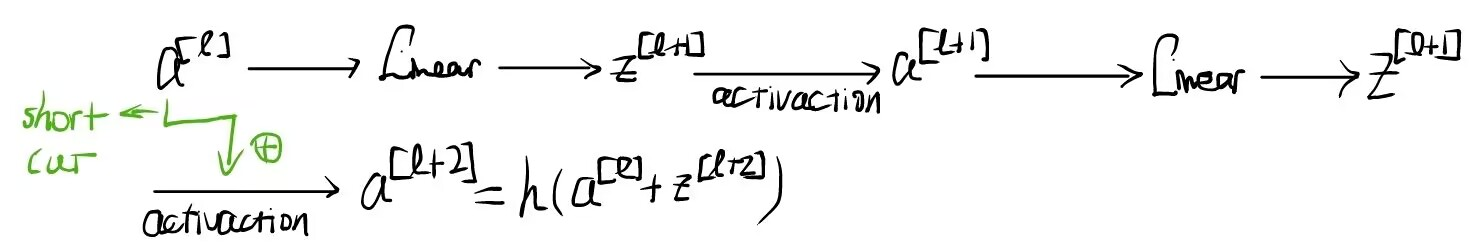
\includegraphics[width=0.7\textwidth]{9.jpg}
	\caption{short cut in RN unit}
\end{figure}
\par Name the following structure as a RN unit
\begin{figure}[htbp]
	\centering
	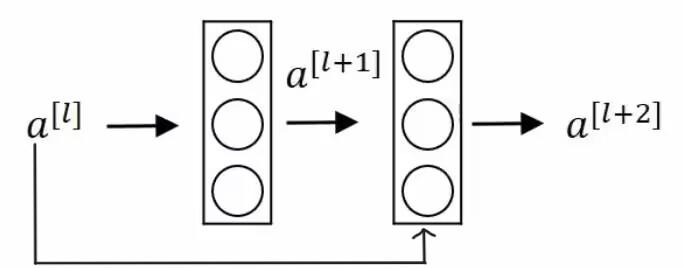
\includegraphics[width=0.7\textwidth]{10.jpg}
	\caption{a RN unit}
\end{figure}
\par Adding RN units is beneficial as in pratice training error goes down monotonely till a plateau while solely using plain network units will decrease training error but increase it as depth of the network increases.(However,theoretically,the training error shall also climb down monotonely.)
\section{1$\times$1 convolution}
1$\times$1 convlution means conducting convolution using filter sized 1$\times$1.Though seemingly silly,it is rather practicle and useful if one wants to reduce multiplication costs while maintaining the whole net working properly.
\par eg. Consider input size = $28\times28\times192$ and every step of convolution using same padding.In first case,there is only one convolutional layer with 32 filters whose size is = $5\times5\times192$.
\begin{figure}[htbp]
	\centering
	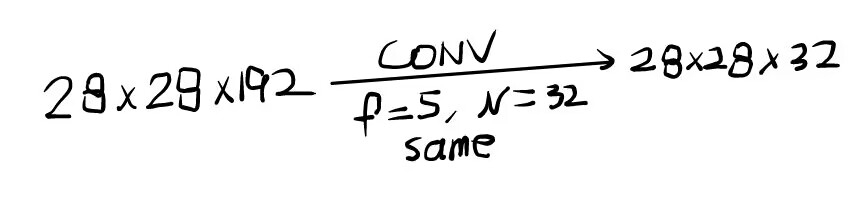
\includegraphics[width=0.6\textwidth]{11.jpg}
	\caption{first canse}
\end{figure}
in this case,total mutiplication costs is $28\times28\times32\times5\times5\times192\approx120M$,a significantly large number.In second case,there are two convolutional layers.First layer is an $1\times1$ CONV layer and second layer is a $5\times5$ CONV layer
\begin{figure}[htbp]
	\centering
	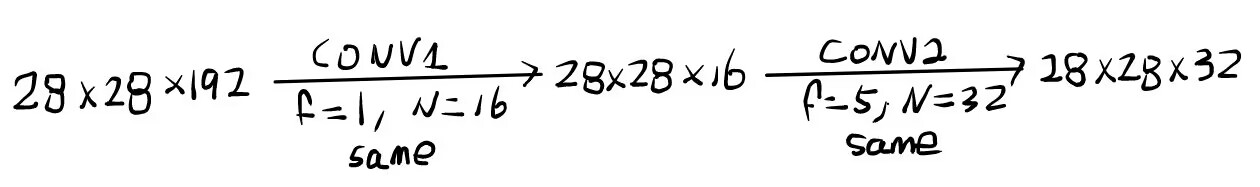
\includegraphics[width=0.6\textwidth]{12.jpg}
	\caption{second canse}
\end{figure}
in this case,the total multiplication costs is $$28\times28\times16\times192+28\times28\times32\times5\times5\times16\approx12.4M$$
which is almost one tenth of that in the first case.
\section{Inception layer}
In an inception layer,certain numbers of feature maps,generated by different filters or pooling+filter,are concatenated together to form a larger feature map.The motivation is that when confused about choosing types of filters,why one just put all the possible case together the same time?
\par eg.Consider input size=$28\times28\times192$ and five CONVs in total.In first CONV,$f_1=3,N_1=32,same\;padding$,in second layer $f_2=5,N_2=32,same \;padding$,in third layer $f_3=6,N_3=16,same \;padding$, and in fourth layer $f_4=4,N_4=16,same\; padding$.In fifth CONV,things are different,it is composite of a pooling and a convolution with $f_5=1,N_5=1,same \;padding$.Each CONV is going to produce a feature map and finally they will be concatenated as a larger feature map sized $28\times28\times144$
\begin{figure}[htbp]
	\centering
	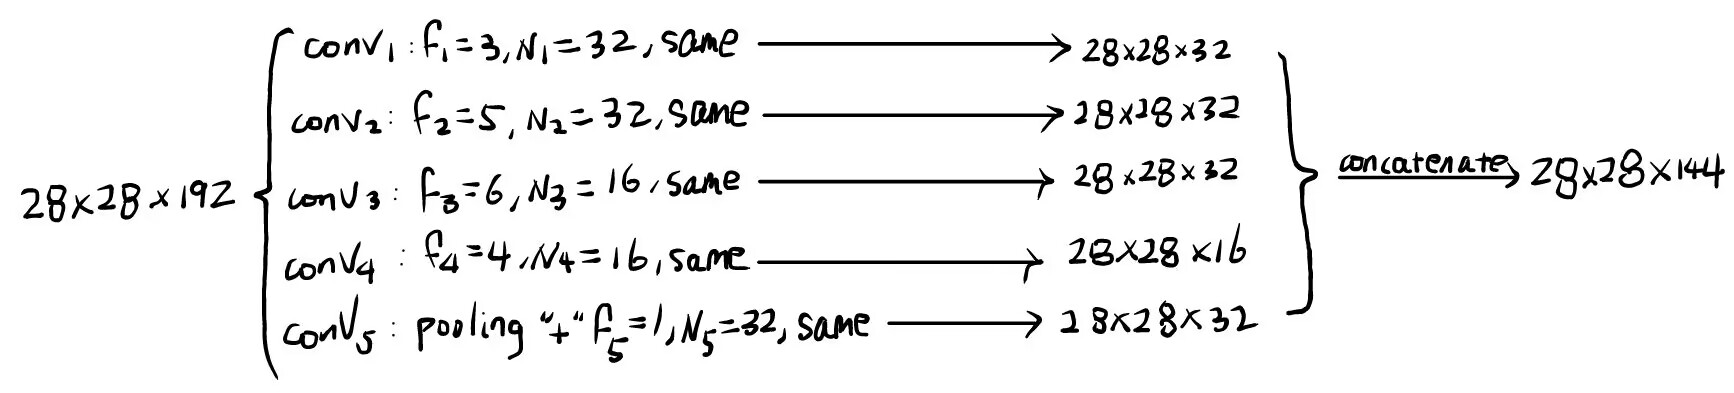
\includegraphics[width=0.7\textwidth]{13.jpg}
	\caption{inception layer}
\end{figure}
\par In actuality,to reduce computational costs,inserting $1\times1$ convolutional steps is frequently considered.
\section{Mobile Net}
Sometimes to save computational resource,Mobile nets are more suitable than usual nets.The spirit of Moblie net is depthwise convolution plus pointwise convolution(1$\times$1 convolution).
\par To make clear comparation,consider input size=$6\times6\times3$ and output size=$4\times4\times5$.If one uses usual CONV,he needs a filter sized $3\times3\times3$ and will consume computational cost of $4\times4\times5\times3\times3\times3=2160$.
\par To perform depthwise convolution,still,filter is needed.But this time,one of the filter in channels is only responsible for one of the channel of input,namely,to convolve filter and input channelwise.So it is obvious that output of this convolution has same number of channels as input.After depthwise convolution comes the $1\times1$ convolution,which involves nothing new.In depth convolution,filter size is $3\times3\times3$ and $1\times1\times3*5$ in $1\times1$ CONV,where $*5$ means there are 5 set of filters.This time,the computational cost is $4\times4\times3\times3\times3+4\times4\times5\times1\times1\times3=672$,which is roughly only 31 percent of that in usual case.
\begin{figure}[htbp]
	\centering
	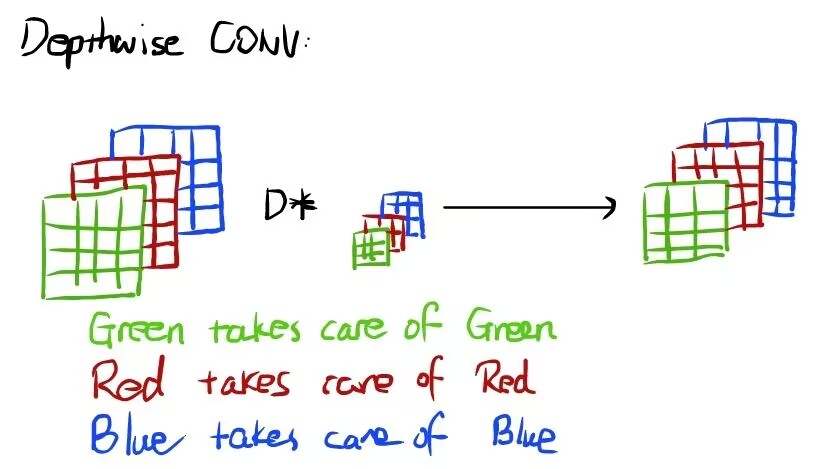
\includegraphics[width=0.7\textwidth]{14.jpg}
	\caption{an example of depthwise convolution}
\end{figure}
\begin{figure}[htbp]
	\centering
	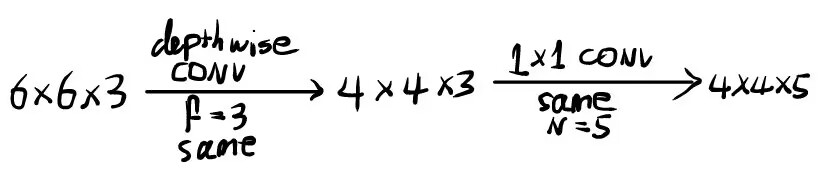
\includegraphics[width=0.7\textwidth]{15.jpg}
	\caption{an example of Mobile net(layer)}
\end{figure}
\end{document}